\documentclass[aspectratio=169, 11pt]{beamer}

% ============================================================
% 基本包
% ============================================================
\usepackage[UTF8]{ctex}
\usepackage{graphicx}
\usepackage{booktabs}
\usepackage{array}
\usepackage{tikz}
\usetikzlibrary{arrows.meta, positioning, shapes.geometric, calc}
\usepackage{fontawesome5}
\usepackage{xcolor}
\usepackage{hyperref}
\usepackage{multicol}

% ============================================================
% 主题设置
% ============================================================
\usetheme{Madrid}
\usecolortheme{whale}
\setbeamertemplate{navigation symbols}{}
\setbeamertemplate{footline}[frame number]
\setbeamerfont{frametitle}{size=\large, series=\bfseries}

% 自定义颜色
\definecolor{mainblue}{RGB}{0, 83, 155}
\definecolor{accentred}{RGB}{204, 51, 51}
\definecolor{accentorange}{RGB}{230, 126, 34}
\definecolor{lightgray}{RGB}{245, 245, 245}
\definecolor{darkgray}{RGB}{60, 60, 60}
\definecolor{successgreen}{RGB}{39, 174, 96}

\setbeamercolor{title}{fg=white, bg=mainblue}
\setbeamercolor{frametitle}{fg=white, bg=mainblue}
\setbeamercolor{block title}{fg=white, bg=mainblue}
\setbeamercolor{block body}{bg=lightgray}
\setbeamercolor{alerted text}{fg=accentred}

% ============================================================
% 文档信息
% ============================================================
\title{面向Agent能力评估的Benchmark数据合成}
\subtitle{文献调研报告 \quad 2024--2026 发展趋势与方法创新}
\author{}
\date{}

% ============================================================
\begin{document}

% ----------------------------------------------------------
% Slide 1: 封面
% ----------------------------------------------------------
\begin{frame}[plain]
\vfill
\begin{center}
{\LARGE\bfseries\color{mainblue} 面向Agent能力评估的\\[6pt]Benchmark数据合成}

\vspace{18pt}
{\large 文献调研报告}

\vspace{8pt}
{\normalsize 2024--2026 发展趋势与方法创新}
\end{center}
\vfill
\end{frame}

% ----------------------------------------------------------
% Slide 2: 为什么Agent需要Benchmark？
% ----------------------------------------------------------
\begin{frame}{为什么Agent需要Benchmark？}
\begin{columns}[T]
\begin{column}{0.55\textwidth}
\textbf{大语言模型 (LLM) $\longrightarrow$ 自主Agent}

\vspace{10pt}
\begin{itemize}
    \item 规划 (Planning)
    \item 推理 (Reasoning)
    \item 工具使用 (Tool Use)
    \item 环境交互 (Interaction)
\end{itemize}
\end{column}
\begin{column}{0.4\textwidth}
\begin{center}
\begin{tikzpicture}[scale=0.8]
\node[draw, rounded corners, fill=mainblue!10, minimum width=2.5cm, minimum height=1cm] (llm) at (0,2) {LLM};
\node[draw, rounded corners, fill=mainblue!30, minimum width=2.5cm, minimum height=1cm] (agent) at (0,0) {自主 Agent};
\draw[-{Stealth[length=3mm]}, thick, mainblue] (llm) -- (agent);
\node[right=0.3cm of agent, text=accentred, font=\large\bfseries] {?};
\end{tikzpicture}

\vspace{6pt}
{\small 如何科学评估？}
\end{center}
\end{column}
\end{columns}

\vspace{12pt}
\begin{block}{}
\centering \textbf{Benchmark = 推动进步的核心引擎}
\end{block}
\end{frame}

% ----------------------------------------------------------
% Slide 3: 手工构建的五大痛点
% ----------------------------------------------------------
\begin{frame}{手工构建的五大痛点}
\small
\begin{tabular}{@{}p{2.8cm}p{8.5cm}@{}}
\toprule
\textbf{痛点} & \textbf{代表性数据} \\
\midrule
标注成本高 & 一条Web Agent轨迹 $\approx$ 数十美元 \\[4pt]
环境搭建难 & OSWorld: 369任务各需定制初始化+评估脚本 \\[4pt]
规模受限 & GAIA: 仅466题 \\[4pt]
过拟合风险 & 静态benchmark易被``记住'' \\[4pt]
领域封闭 & 医疗/法律/金融缺乏benchmark \\
\bottomrule
\end{tabular}

\vspace{12pt}
\begin{center}
\alert{\large $\Longrightarrow$ 核心矛盾：需求增长 $\gg$ 手工产能}
\end{center}
\end{frame}

% ----------------------------------------------------------
% Slide 4: 早期手工Benchmark概览
% ----------------------------------------------------------
\begin{frame}{早期手工Benchmark概览}
\small
\begin{tabular}{@{}lp{7.5cm}@{}}
\toprule
\textbf{Benchmark} & \textbf{关键发现} \\
\midrule
AgentBench \scriptsize{(ICLR'24)} & 8环境$\times$27模型 $\rightarrow$ 开源vs闭源差距巨大 \\[4pt]
WebArena \scriptsize{(ICLR'24)} & GPT-4: 14.41\% \; vs \; 人类: 78.24\% \\[4pt]
OSWorld \scriptsize{(NeurIPS'24)} & 首个真实OS级环境 (Ubuntu/Win/macOS) \\[4pt]
GAIA \scriptsize{(ICLR'24)} & 466题 $\rightarrow$ ``人类简单但AI极难'' \\[4pt]
SWE-bench \scriptsize{(ICLR'24)} & 真实GitHub Issue $\rightarrow$ 代码修复评估 \\
\bottomrule
\end{tabular}

\vspace{10pt}
\begin{center}
\textit{这些经典benchmark定义了评估标准，但全是手工堆出来的。}
\end{center}
\end{frame}

% ----------------------------------------------------------
% Slide 5: 手工Benchmark的教训
% ----------------------------------------------------------
\begin{frame}{手工Benchmark的教训}
\begin{itemize}
    \setlength\itemsep{8pt}
    \item \textbf{AgentBench} $\longrightarrow$ 8个环境全人工设计，难扩展到新领域
    \item \textbf{WebArena} $\longrightarrow$ 每个任务需手工写初始状态 + 评估脚本
    \item \textbf{OSWorld} $\longrightarrow$ 369个任务 = 369套初始化 + 评估逻辑
    \item \textbf{GAIA} $\longrightarrow$ 466题精心设计，但规模已达瓶颈
\end{itemize}

\vspace{16pt}
\begin{block}{结论}
\centering 手工方法已经走到了尽头，\alert{自动化合成是唯一出路}。
\end{block}
\end{frame}

% ----------------------------------------------------------
% Slide 6: 方法论反思：AI Agents That Matter
% ----------------------------------------------------------
\begin{frame}{方法论反思：AI Agents That Matter}
\textbf{AI Agents That Matter} \quad {\small (Kapoor et al., 2024)}

\vspace{10pt}
指出的四大缺陷：
\begin{enumerate}
    \setlength\itemsep{6pt}
    \item 过度关注准确率，忽略\alert{成本--收益}评估
    \item 需求定义混淆（benchmark $\neq$ 产品需求）
    \item Holdout集不足 $\rightarrow$ 过拟合
    \item 缺乏标准化评估协议
\end{enumerate}

\vspace{12pt}
\begin{center}
$\Longrightarrow$ \textbf{为后续所有数据合成工作设定了方法论约束}
\end{center}
\end{frame}

% ----------------------------------------------------------
% Slide 7: 分割页 — 第一部分：轨迹合成
% ----------------------------------------------------------
\begin{frame}[plain]
\vfill
\begin{center}
{\large\color{gray} 第一部分}

\vspace{8pt}
{\LARGE\bfseries\color{mainblue} 轨迹合成}

\vspace{12pt}
{\normalsize 从人工标注到自动生成}

\vspace{16pt}

\begin{tikzpicture}
\draw[mainblue, thick] (-4,0) -- (4,0);
\end{tikzpicture}

\vspace{10pt}
{\small\textit{核心问题：如何在保证质量的前提下，低成本、大规模地\\生成Agent执行任务的完整操作记录？}}
\end{center}
\vfill
\end{frame}

% ----------------------------------------------------------
% Slide 8: ToolLLM → APIGen：验证的革命
% ----------------------------------------------------------
\begin{frame}{ToolLLM $\rightarrow$ APIGen：验证的革命}
\begin{columns}[T]
\begin{column}{0.48\textwidth}
\textbf{ToolLLM} {\scriptsize (NeurIPS 2023)}
\begin{itemize}
    \small
    \item 16,464个真实API
    \item ChatGPT生成指令
    \item DFS搜索标注路径
    \item[\color{accentred}\textbullet] \color{accentred} 问题：LLM既生成又验证
\end{itemize}
\end{column}
\begin{column}{0.48\textwidth}
\textbf{APIGen} {\scriptsize (Salesforce, 2024)}

\textbf{三层可执行验证：}
\begin{enumerate}
    \small
    \item 格式检查 (JSON/类型/参数)
    \item 实际执行 (真实API调用)
    \item 语义验证 (LLM判定意图)
\end{enumerate}
\end{column}
\end{columns}

\vspace{10pt}
\begin{block}{关键数据}
\begin{itemize}
    \item 过滤率：\alert{40\%--60\%} 的LLM生成数据被淘汰
    \item 结果：7B模型 $>$ 多个GPT-4版本 (BFCL)；1B模型 $>$ GPT-3.5 + Claude-3 Haiku
\end{itemize}
\end{block}
\end{frame}

% ----------------------------------------------------------
% Slide 9: AgentTrek：教程引导的轨迹合成
% ----------------------------------------------------------
\begin{frame}{AgentTrek：教程引导的轨迹合成}
{\small ICLR 2025 Spotlight $\cdot$ HKU / Salesforce}

\vspace{6pt}
\textbf{核心洞察：}互联网 ``How to'' 教程 = 免费任务知识！

\vspace{8pt}
\textbf{三阶段管线：}
\begin{enumerate}
    \item 自动收集教程 $\rightarrow$ 分类器过滤高质量文本
    \item 转化为结构化任务规范（步骤级指令）
    \item VLM Agent按教程执行 + VLM评估器验证
\end{enumerate}

\vspace{8pt}
\textbf{关键创新：「引导回放」} --- Agent在教程帮助下执行，比自主探索可靠得多

\vspace{10pt}
\begin{block}{成本革命}
\centering \alert{\$0.55/条} \; vs \; 人工 \$10+/条 $\longrightarrow$ 降低1--2个数量级
\end{block}
\end{frame}

% ----------------------------------------------------------
% Slide 10: Agent-as-Annotators：数据效率的极限
% ----------------------------------------------------------
\begin{frame}{Agent-as-Annotators：数据效率的极限}
{\small McGill / Mila $\cdot$ 2026}

\vspace{4pt}
\textbf{``将轨迹合成类比为人工标注流水线''}

\vspace{4pt}
\begin{center}
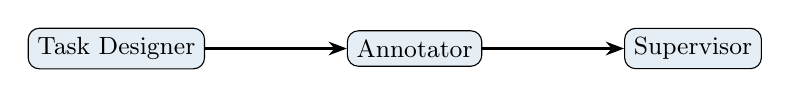
\begin{tikzpicture}[node distance=1.8cm, every node/.style={font=\small}]
\node[draw, rounded corners, fill=mainblue!10] (td) {Task Designer};
\node[draw, rounded corners, fill=mainblue!10, right=of td] (ann) {Annotator};
\node[draw, rounded corners, fill=mainblue!10, right=of ann] (sup) {Supervisor};
\draw[-{Stealth}, thick] (td) -- (ann);
\draw[-{Stealth}, thick] (ann) -- (sup);
\end{tikzpicture}
\end{center}

\vspace{2pt}
\textbf{两大创新：} Evaluation Hints + 推理链蒸馏（做什么 + 为什么）

\vspace{6pt}
\begin{columns}[T]
\begin{column}{0.45\textwidth}
\small
生成 3,000 条\\
过滤保留 \textbf{2,322 条} (77.4\%)
\end{column}
\begin{column}{0.5\textwidth}
\small
\textbf{WebArena 成功率：}\\
\alert{41.5\%} --- 9B Student Model\\
36.0\% --- Claude 3.5 Sonnet\\
31.5\% --- GPT-4o\\
21.7\% --- 此前最佳开源
\end{column}
\end{columns}

\vspace{4pt}
\begin{center}
\small 跨环境泛化：WorkArena L1 上 \textbf{+18.2 pp}
\end{center}
\end{frame}

% ----------------------------------------------------------
% Slide 11: 轨迹合成小结
% ----------------------------------------------------------
\begin{frame}{轨迹合成小结}
\textbf{发展脉络：}

\vspace{6pt}
\begin{center}
\begin{tikzpicture}[node distance=0.8cm, every node/.style={font=\small}]
\node[draw, rounded corners, fill=mainblue!8] (t1) {ToolLLM};
\node[draw, rounded corners, fill=mainblue!15, right=0.6cm of t1] (t2) {APIGen};
\node[draw, rounded corners, fill=mainblue!22, right=0.6cm of t2] (t3) {AgentTrek};
\node[draw, rounded corners, fill=mainblue!30, right=0.6cm of t3] (t4) {Agent-as-Annot.};
\draw[-{Stealth}, thick] (t1) -- (t2);
\draw[-{Stealth}, thick] (t2) -- (t3);
\draw[-{Stealth}, thick] (t3) -- (t4);
\node[below=0.2cm of t1, font=\tiny, text=gray] {LLM幻觉};
\node[below=0.2cm of t2, font=\tiny, text=gray] {三重验证};
\node[below=0.2cm of t3, font=\tiny, text=gray] {\$0.55/条};
\node[below=0.2cm of t4, font=\tiny, text=gray] {2322条$>$GPT-4o};
\end{tikzpicture}
\end{center}

\vspace{12pt}
\textbf{核心趋势：}
\begin{enumerate}
    \item \textbf{验证：} LLM自判 $\rightarrow$ 可执行验证 \quad {\small (必然方向)}
    \item \textbf{知识源：} 模型生成 $\rightarrow$ 互联网教程 $\rightarrow$ 强模型蒸馏
    \item \textbf{成本：} \$10+/条 $\rightarrow$ \$0.55/条 \quad {\small (2个数量级)}
    \item \textbf{效率：} 数量 $\rightarrow$ 质量 \quad {\small (关键翻转)}
\end{enumerate}
\end{frame}

% ----------------------------------------------------------
% Slide 12: 分割页 — 第二部分：环境合成
% ----------------------------------------------------------
\begin{frame}[plain]
\vfill
\begin{center}
{\large\color{gray} 第二部分}

\vspace{8pt}
{\LARGE\bfseries\color{mainblue} 环境合成}

\vspace{12pt}
{\normalsize 从``造数据''到``造世界''}

\vspace{16pt}

\begin{tikzpicture}
\draw[mainblue, thick] (-4,0) -- (4,0);
\end{tikzpicture}

\vspace{10pt}
{\small\textit{核心思路转变：与其让LLM模仿人的行为，\\不如让LLM创造一个世界，让Agent自己在里面学。}}
\end{center}
\vfill
\end{frame}

% ----------------------------------------------------------
% Slide 13: EnvScaler & AWM：程序化环境生成
% ----------------------------------------------------------
\begin{frame}{EnvScaler \& AWM：程序化环境生成}
\begin{columns}[T]
\begin{column}{0.48\textwidth}
\textbf{EnvScaler} {\scriptsize (人大, 2026)}

\begin{itemize}
    \small
    \item SkelBuilder: 挖掘真实主题 $\rightarrow$ 设计API/数据模型
    \item ScenGenerator: 生成任务场景 + 规则验证函数
    \item 产出：191环境 + $\sim$7,000场景
\end{itemize}
\end{column}
\begin{column}{0.48\textwidth}
\textbf{AWM} {\scriptsize (Snowflake, 2026)}

\begin{itemize}
    \small
    \item LLM规划 $\rightarrow$ 生成可执行代码
    \item 每个环境 $\approx$ 35个工具
    \item DB状态直接计算奖励
    \item 产出：1,000个环境
\end{itemize}
\end{column}
\end{columns}

\vspace{10pt}
\begin{block}{vs 纯LLM模拟环境}
\centering
\small
\begin{tabular}{lccc}
 & 状态一致 & 可重现性 & 奖励可靠性 \\
\midrule
程序化/DB & \color{successgreen}\checkmark & \color{successgreen}\checkmark & \color{successgreen}\checkmark \\
纯LLM模拟 & \color{accentred}$\times$ & \color{accentred}$\times$ & \color{accentred}$\times$ \\
\end{tabular}
\end{block}

\vspace{4pt}
\begin{center}
\small\textbf{关键结果：}纯合成环境训练的Agent，在真实Benchmark上表现优秀
\end{center}
\end{frame}

% ----------------------------------------------------------
% Slide 14: VeriEnv：用LLM克隆真实网站
% ----------------------------------------------------------
\begin{frame}{VeriEnv：用LLM克隆真实网站}
{\small Georgia Tech $\cdot$ 2026}

\vspace{6pt}
\textbf{核心思路：}让LLM克隆真实网站为可执行复制品

\vspace{8pt}
\begin{center}
\begin{tikzpicture}[node distance=1.5cm, every node/.style={font=\small}]
\node[draw, rounded corners, fill=accentorange!15] (real) {真实网站};
\node[draw, rounded corners, fill=mainblue!15, right=2cm of real] (clone) {克隆复制品};
\node[draw, rounded corners, fill=successgreen!15, right=2cm of clone] (sdk) {Python SDK};
\draw[-{Stealth}, thick] (real) -- node[above, font=\scriptsize]{LLM分析} (clone);
\draw[-{Stealth}, thick] (clone) -- node[above, font=\scriptsize]{配备} (sdk);
\end{tikzpicture}
\end{center}

\vspace{6pt}
\textbf{Python SDK 能力：}
\begin{itemize}
    \small
    \item 读取数据库状态 / 获取会话信息
    \item 编程式验证任务完成
    \item 奖励信号\textbf{完全确定性}（无LLM随机性）
\end{itemize}

\vspace{8pt}
\begin{block}{重要发现}
\centering 增加克隆网站数 $\rightarrow$ 持续性能提升 $\rightarrow$ 暗示\textbf{``环境层面的 Scaling Law''}
\end{block}
\end{frame}

% ----------------------------------------------------------
% Slide 15: Environment Tuning：范式转移
% ----------------------------------------------------------
\begin{frame}{Environment Tuning：范式转移}
{\small 蚂蚁 + 浙大 $\cdot$ ICLR 2026}

\vspace{4pt}
\textbf{核心论断：不要只调Agent，调环境！}

\vspace{6pt}
\textbf{三重环境增强：}
\begin{enumerate}
    \small
    \item \textbf{结构化课程} --- 从简到难的任务渐进
    \item \textbf{可操作增强} --- 犯错时环境提供纠正性反馈
    \item \textbf{细粒度奖励} --- 步骤级 + 状态匹配级（非二进制）
\end{enumerate}

\vspace{6pt}
实验设置：\textbf{仅 400 个问题实例，无专家轨迹}

\vspace{6pt}
\small
\begin{tabular}{lcc}
\toprule
 & In-Distribution & Out-of-Distribution \\
\midrule
SFT on synthetic traces & 好 & \color{accentred}严重退化 \\
Environment Tuning & 竞争力 & \color{successgreen}\textbf{显著最优} \\
\bottomrule
\end{tabular}

\vspace{8pt}
\begin{center}
\alert{核心发现：SFT在合成数据上过拟合！数据使用方式 $>$ 数据本身}
\end{center}
\end{frame}

% ----------------------------------------------------------
% Slide 16: gg-bench：Benchmark即生成过程
% ----------------------------------------------------------
\begin{frame}{gg-bench：Benchmark即生成过程}
{\small UC Berkeley $\cdot$ 2025}

\vspace{6pt}
\textbf{理念：}Benchmark = 数据\textbf{生成过程}，而非静态数据集

\vspace{8pt}
\textbf{三阶段生成管线：}
\begin{enumerate}
    \item LLM生成全新游戏描述
    \item LLM实现为可执行Gym环境
    \item 自我对弈RL $\rightarrow$ 训练最优对手
\end{enumerate}

\vspace{8pt}
\textbf{评估方式：}Agent vs RL最优对手 $\rightarrow$ 胜率评分

\vspace{8pt}
\begin{columns}[T]
\begin{column}{0.45\textwidth}
\small
\textbf{结果：}\\
GPT-4o / Claude 3.7: \alert{7\%--9\%}\\
o1 / o3-mini: \textbf{31\%--36\%}
\end{column}
\begin{column}{0.5\textwidth}
\small
\textbf{根本优势：}\\
每次生成新游戏\\
$\rightarrow$ 永不饱和\\
$\rightarrow$ \alert{根治过拟合}
\end{column}
\end{columns}
\end{frame}

% ----------------------------------------------------------
% Slide 17: 分割页 — 第三部分：集成范式
% ----------------------------------------------------------
\begin{frame}[plain]
\vfill
\begin{center}
{\large\color{gray} 第三部分}

\vspace{8pt}
{\LARGE\bfseries\color{mainblue} 集成范式}

\vspace{12pt}
{\normalsize 将所有环节串成一个闭环}

\vspace{16pt}
\begin{tikzpicture}[node distance=0.6cm, every node/.style={font=\small, draw, rounded corners, minimum height=0.7cm, fill=mainblue!10}]
\node (t1) {任务合成};
\node[right=of t1] (t2) {环境执行};
\node[right=of t2] (t3) {验证评估};
\node[right=of t3] (t4) {策略学习};
\draw[-{Stealth}, thick] (t1) -- (t2);
\draw[-{Stealth}, thick] (t2) -- (t3);
\draw[-{Stealth}, thick] (t3) -- (t4);
\draw[-{Stealth}, thick, mainblue] (t4.south) -- ++(0,-0.6) -| (t1.south);
\end{tikzpicture}
\end{center}
\vfill
\end{frame}

% ----------------------------------------------------------
% Slide 18: EvoCUA：自我进化的终极闭环
% ----------------------------------------------------------
\begin{frame}{EvoCUA：自我进化的终极闭环}
{\small 阿里 $\cdot$ 2026 --- 当前最高集成度}

\vspace{6pt}
\textbf{三组件闭环：}
\begin{enumerate}
    \item \textbf{可验证合成引擎} --- 自主生成任务 + 可执行验证器
    \item \textbf{万级异步沙箱基础设施} --- 数万沙箱并行rollout
    \item \textbf{迭代进化学习} --- 成功轨迹强化 + 失败轨迹利用
\end{enumerate}

\vspace{10pt}
\begin{block}{OSWorld 结果}
\centering
\begin{tabular}{lc}
EvoCUA & \alert{\textbf{56.7\%}} \quad (新 SOTA) \\
UI-TARS-2 (闭源) & 53.1\% \\
OpenCUA-72B (此前最佳开源) & 45.0\% \\
\end{tabular}
\end{block}

\vspace{6pt}
\begin{center}
\textit{本质：自我维持的进化循环 --- 数据合成不再是一次性行为，\\而是持续进化的生命过程。}
\end{center}
\end{frame}

% ----------------------------------------------------------
% Slide 19: EigenData：基准审计与全生命周期
% ----------------------------------------------------------
\begin{frame}{EigenData：基准审计与全生命周期}
{\small Amazon $\cdot$ 2026}

\vspace{4pt}
\textbf{多Agent协作平台：}

\vspace{2pt}
\begin{center}
\begin{tikzpicture}[every node/.style={font=\small, draw, rounded corners}]
\node[fill=mainblue!20] (core) at (0,0) {EigenCore (顶层协调)};
\node[fill=mainblue!8] (db) at (-3,-1.2) {DatabaseAgent};
\node[fill=mainblue!8] (code) at (0,-1.2) {CodingAgent};
\node[fill=mainblue!8] (data) at (3,-1.2) {DataAgent};
\draw[-{Stealth}] (core) -- (db);
\draw[-{Stealth}] (core) -- (code);
\draw[-{Stealth}] (core) -- (data);
\end{tikzpicture}
\end{center}

\vspace{4pt}
\textbf{重要贡献：对 BFCL-V3 进行全面审计}
\begin{itemize}
    \small
    \item 发现系统性错误：schema不一致、实现偏差、评估指标误导
    \item 提出\textbf{「结果感知评估」}：不看轨迹匹配 $\rightarrow$ 看数据库最终状态
    \item 模型排名与人类判断相关性\textbf{显著更高}
\end{itemize}
\end{frame}

% ----------------------------------------------------------
% Slide 20: 全景对比
% ----------------------------------------------------------
\begin{frame}{全景对比}
\centering
\scriptsize
\begin{tabular}{@{}llll@{}}
\toprule
\textbf{方法} & \textbf{合成什么} & \textbf{核心验证方式} & \textbf{关键指标} \\
\midrule
APIGen & 函数调用数据 & 三层可执行验证 & 7B $>$ GPT-4 \\
AgentTrek & Web轨迹+推理链 & VLM评估器 & \$0.55/条 \\
Agent-as-Annot. & 推理链轨迹 & LLM Judge+hints & 2.3K$\rightarrow$41.5\% \\
EnvScaler & 环境+验证函数 & 规则验证函数 & 191环境 \\
AWM & 环境+DB+奖励 & DB状态对比 & 1000环境 \\
VeriEnv & 克隆网站+SDK & Python SDK验证 & 持续scaling \\
Env.\ Tuning & 增强环境奖励 & 进度奖励 & 400实例,OOD最优 \\
gg-bench & 动态游戏环境 & RL对手胜率 & 根治过拟合 \\
EvoCUA & 任务+验证器+轨迹 & 可执行验证+沙箱 & 56.7\% OSWorld \\
EigenData & DB+环境+轨迹 & 结果感知评估 & Benchmark审计 \\
\bottomrule
\end{tabular}

\vspace{8pt}
\small
\textit{验证方式持续升级：LLM自判 $\rightarrow$ 可执行 $\rightarrow$ 规则 $\rightarrow$ DB/SDK $\rightarrow$ 确定性编程验证}
\end{frame}

% ----------------------------------------------------------
% Slide 21: 五大技术趋势
% ----------------------------------------------------------
\begin{frame}{五大技术趋势}
\begin{enumerate}
    \setlength\itemsep{7pt}
    \item \textbf{验证方式进化}\\
    {\small LLM-as-Judge $\rightarrow$ 实际执行 $\rightarrow$ 程序化/DB/SDK $\rightarrow$ 可执行验证成为标配}

    \item \textbf{合成粒度升级}\\
    {\small 指令 $\rightarrow$ 轨迹 $\rightarrow$ 环境 $\rightarrow$ 完整生态 \quad (EvoCUA = 终极形态)}

    \item \textbf{质量 $\gg$ 数量}\\
    {\small 2.3K轨迹 $>$ GPT-4o \;\;|\;\; 400实例竞争力 \;\;|\;\; 10网站匹配大量人工数据}

    \item \textbf{静态 $\rightarrow$ 动态自进化}\\
    {\small gg-bench ``生成即评估'' + EvoCUA 持续闭环 $\rightarrow$ 永不饱和}

    \item \textbf{合成环境 $>$ 合成数据} {\small (范式级转向)}\\
    {\small Environment Tuning: 造好环境比造好数据更重要；SFT过拟合警示}
\end{enumerate}
\end{frame}

% ----------------------------------------------------------
% Slide 22: 挑战与未来
% ----------------------------------------------------------
\begin{frame}{挑战与未来}
\begin{enumerate}
    \setlength\itemsep{8pt}
    \item \textbf{计算成本与可及性}\\
    {\small EvoCUA级``万级沙箱'' $\rightarrow$ 学术界能否承受？}

    \item \textbf{真实性---可扩展性光谱}\\
    {\small 高真实 $\leftarrow$ VeriEnv(克隆) $\cdot$ OSWorld(真OS) $\cdot$ EnvScaler $\cdot$ AWM(1000环境) $\rightarrow$ 高扩展}\\
    {\small 最优点在哪？开放问题。}

    \item \textbf{理论基础缺失}\\
    {\small 合成数据的统计特性？泛化界？目前几乎全部实验驱动。}

    \item \textbf{评估的``元问题''}\\
    {\small EigenData发现：人工标注的benchmark也有系统性错误}\\
    {\small $\rightarrow$ 谁来评估评估者？自动化审计应成为标准流程。}
\end{enumerate}
\end{frame}

% ----------------------------------------------------------
% Slide 23: Thank You & Q&A
% ----------------------------------------------------------
\begin{frame}[plain]
\vfill
\begin{center}
{\Huge\bfseries\color{mainblue} Thank You!}

\vspace{20pt}
{\large 面向Agent能力评估的Benchmark数据合成}

\vspace{6pt}
{\normalsize 2024--2026 文献调研}

\vspace{24pt}
{\Large 欢迎提问}
\end{center}
\vfill
\end{frame}

\end{document}
